%%% タイトル howtoketmathLMS
\documentclass[landscape,10pt]{ujarticle}
\special{papersize=\the\paperwidth,\the\paperheight}
\usepackage{ketpic,ketlayer}
\usepackage{ketslide}
\usepackage{amsmath,amssymb}
\usepackage{bm,enumerate}
\usepackage[dvipdfmx]{graphicx}
\usepackage{color}
\definecolor{slidecolora}{cmyk}{0.98,0.13,0,0.43}
\definecolor{slidecolorb}{cmyk}{0.2,0,0,0}
\definecolor{slidecolorc}{cmyk}{0.2,0,0,0}
\definecolor{slidecolord}{cmyk}{0.2,0,0,0}
\definecolor{slidecolore}{cmyk}{0,0,0,0.5}
\definecolor{slidecolorf}{cmyk}{0,0,0,0.5}
\definecolor{slidecolori}{cmyk}{0.98,0.13,0,0.43}
\def\setthin#1{\def\thin{#1}}
\setthin{0}
\newcommand{\slidepage}[1][s]{%
\setcounter{ketpicctra}{18}%
\if#1m \setcounter{ketpicctra}{1}\fi
\hypersetup{linkcolor=black}%

\begin{layer}{118}{0}
\putnotee{122}{-\theketpicctra.05}{\small\thepage/\pageref{pageend}}
\end{layer}\hypersetup{linkcolor=blue}

}
\usepackage[dvipdfmx]{pict2e}
\usepackage{pict2e}
\usepackage[dvipdfmx,colorlinks=true,linkcolor=blue,filecolor=blue]{hyperref}

\setmargin{25}{145}{15}{100}

\ketslideinit

\pagestyle{empty}

\begin{document}

\begin{layer}{120}{0}
\putnotese{0}{0}{{\Large\bf
\color[cmyk]{1,1,0,0}

\begin{layer}{120}{0}
{\Huge \putnotes{60}{20}{KeTMath使い方}}
\putnotes{60}{50}{高遠節夫}
\putnotes{60}{60}{\ketcindy センター}
\putnotes{60}{70}{2021.10.27}
\end{layer}

}
}
\end{layer}

\def\mainslidetitley{22}
\def\ketcletter{slidecolora}
\def\ketcbox{slidecolorb}
\def\ketdbox{slidecolorc}
\def\ketcframe{slidecolord}
\def\ketcshadow{slidecolore}
\def\ketdshadow{slidecolorf}
\def\slidetitlex{6}
\def\slidetitlesize{1.3}
\def\mketcletter{slidecolori}
\def\mketcbox{yellow}
\def\mketdbox{yellow}
\def\mketcframe{yellow}
\def\mslidetitlex{62}
\def\mslidetitlesize{2}

\color{black}
\normalsize\bf\boldmath
\addtocounter{page}{-1}

\def\rad{\;\mathrm{rad}}
\newcommand{\hako}[2][6mm]{\fbox{$\mathstrut$\Ctab{#1}{#2}}}
\newcommand{\dint}{\displaystyle\int}
\newcommand{\dlim}{\displaystyle\lim}
\newcommand{\dc}{: \hspace{-1.4mm}:}
\setmargin{25}{150}{15}{100}%
%%%%%%%%%%%%

%%%%%%%%%%%%%%%%%%%%

\mainslide{数式の簡易記法とKeTMath}


%%repeat=4,para
\slidepage[m]
%%%%%%%%%%%%

%%%%%%%%%%%%%%%%%%%%

\newslide{数式の簡易記法1}

\vspace*{18mm}

%%repeat=4,para
\slidepage
\begin{itemize}
\item
\Ltab{4.5zw}{分数}$\dfrac{a}{b}\ \Longrightarrow$\ \verb|fr(a,b)|,\ \verb|(a)/(b)|
  注)小さい分数 \verb|tfr(a,b)|\vspace{-2mm}
\item
\Ltab{4.5zw}{掛け算}$ab\ \Longrightarrow$\ \verb|ab|  注)\verb|a*b|も可\vspace{-2mm}
\item
\Ltab{4.5zw}{べき乗}$a^b\ \Longrightarrow$\ \verb|a^(b)|  注)bが1文字の場合は \verb|a^b|も可\vspace{-2mm}
\item
\Ltab{4.5zw}{べき乗根}$\sqrt{a},\ \sqrt[3]{a}\ \Longrightarrow$\ \verb|sq(a), sq(3,a)|\vspace{-2mm}
\item
\Ltab{4.5zw}{三角関数}$\sin x, \sin^2x\ \Longrightarrow$\ \verb|sin(x), sin(2,x)|\vspace{-2mm}
\item
\Ltab{4.5zw}{度}$60{}^{\circ}\ \Longrightarrow$\ \verb|60(deg)|\vspace{-2mm}
\item
\Ltab{4.5zw}{円周率}$\pi \ \Longrightarrow$\ \verb|pi|\vspace{-2mm}
\item
\Ltab{4.5zw}{対数関数}$\log x, \log_a x, \ln x \Longrightarrow$\ \verb|log(x), log(a,x), ln(x)|\vspace{-2mm}
\item
\Ltab{4.5zw}{改行}//\vspace{-2mm}
\item
\Ltab{4.5zw}{スペース}\ (sp)  注)\TeX の\verb|\;|を出力\vspace{-2mm}
\item
\Ltab{4.5zw}{立体}$100\text{m}\ \Longrightarrow$\ \verb|100tx(m)|\vspace{-2mm}
%%item::\Ltab{4.5zw}{立体} $\text{cosh}\ x \ \Longrightarrow$\ \verb|tx(cosh)(sp)x| 注)\TeX 記号\verb|\cosh(sp)x|も可\vspace{-2mm}
\end{itemize}
%%%%%%%%%%%%

%%%%%%%%%%%%%%%%%%%%

\newslide{数式の簡易記法2}

\vspace*{18mm}

%%repeat=4,para
\slidepage

\begin{layer}{120}{0}
\putnotese{76}{22}{\small\fbox{%%
\begin{tabular}{l}
(\ ) は自動判定するが,強制的に\\
 (\ )を外すとき式の先頭に !\\
 (\ )をつけるとき式の先頭に !!\\
   int(!x+y,x)
\end{tabular}
}}
\end{layer}

\begin{itemize}
\item
\Ltab{4.5zw}{積分}$\dint x^2\,dx,\ \dint_a^b x^2\,dx \ \Longrightarrow$\ \verb|int(x^2,x), int(a,b,x^2,x)|\vspace{-2mm}
\item
\Ltab{6zw}{ブラケット}$\Bigl[f(x)\Bigr]_a^b\  \Longrightarrow$\ \verb|br(f(x),a,b)|\vspace{-2mm}
\item
\Ltab{4.5zw}{極限}$\dlim_{x \to a}f(x) \ \Longrightarrow$\  \verb|lim(x,a,f(x))|\vspace{-2mm}
\item
\Ltab{4.5zw}{和}$\displaystyle\sum_{k=1}^{n}k^2 \ \Longrightarrow$\  \verb|sum(k=1,n,k^2)|\vspace{-2mm}
\item
\Ltab{7zw}{微分・偏微分}$\dfrac{dy}{dx},\ \dfrac{\partial z}{\partial x} \ \Longrightarrow$\ \verb|diff(y,x)|, \verb|par(z,x)|
\item
\Ltab{7zw}{行列・行列式}$\begin{pmatrix}a&b\\c&d\end{pmatrix},\ \left|\begin{array}{cc}a&b\\c&d\end{array}\right|
\ \Longrightarrow$\ \verb|mat(a,b;c,d)|, \verb|det(a,b;c,d)|\vspace{-2mm}
\item
\Ltab{4.5zw}{場合分け}$\begin{cases}a&(x<0)\\c&(x \geq 0)\end{cases} \ \Longrightarrow$\ \verb|case(a,(x<0);c,(x(geq)0))|\vspace{-2mm}
\end{itemize}
%%%%%%%%%%%%

%%%%%%%%%%%%%%%%%%%%

\newslide{数式の簡易記法3}

\vspace*{18mm}

%%repeat=4,para
\slidepage
\begin{itemize}
\item
\Ltab{8zw}{ドットなど}$\cdot,\ \times\ \Longrightarrow$\ \verb|(dot), (cross)|\vspace{-2mm}
\item
\Ltab{8zw}{複号}$\pm, \mp\ \Longrightarrow$\ \verb|(pm), (mp)|\vspace{-2mm}
\item
\Ltab{8zw}{不等号}$<, >, \leq, \geq\ \Longrightarrow$\ \verb|<, >, (leq), (geq)|\vspace{-2mm}
\item
\Ltab{8zw}{下添字}$a_n\ \Longrightarrow$\ \verb|a_n|\vspace{-2mm}
\item
全角文字を混ぜてもよい\\
 $x^2+2x-3=0$の解は$x=1,-3\ \Longrightarrow$\ \verb|x^2+2x-3=0の解はx=1,-3|\vspace{-2mm}
\item
\Ltab{8zw}{ギリシャ文字}$\alpha, \beta\ \Longrightarrow$\ \verb|{\alpha},{\beta}|\vspace{-2mm}
\item
その他の\TeX 記号はそのまま書いて(sp)で区切る\\
 $\sim, \subset, \in  \Longrightarrow$\ \verb|\sim(sp)\subset(sp)\in|\vspace{-2mm}
\item
Maxima数式に変換する場合,数式文字は1文字とする.\\
 absin(x)\ $\Longrightarrow \ $(Maxima数式) \verb|a*b*sin(x)| \vspace{-2mm}
\end{itemize}
%%%%%%%%%%%%

%%%%%%%%%%%%%%%%%%%%

\newslide{KeTMath(数式入力アプリ)}

\vspace*{18mm}

%%repeat=4,para
\slidepage
\begin{itemize}
\item
{\footnotesize\url{https://s-takato.github.io/ketcindysample/ketmath/offline/ketmathjsoffL.html}}\\
 ・samples of ketcindy  $>$ ketmath systemに行けばよい.
\item
キーボードにより簡易数式を入力することができる\\
 ・\TeX 数式(TeXボタンを押すとソースも)が表示される.

\begin{layer}{120}{0}
\putnotes{52}{2}{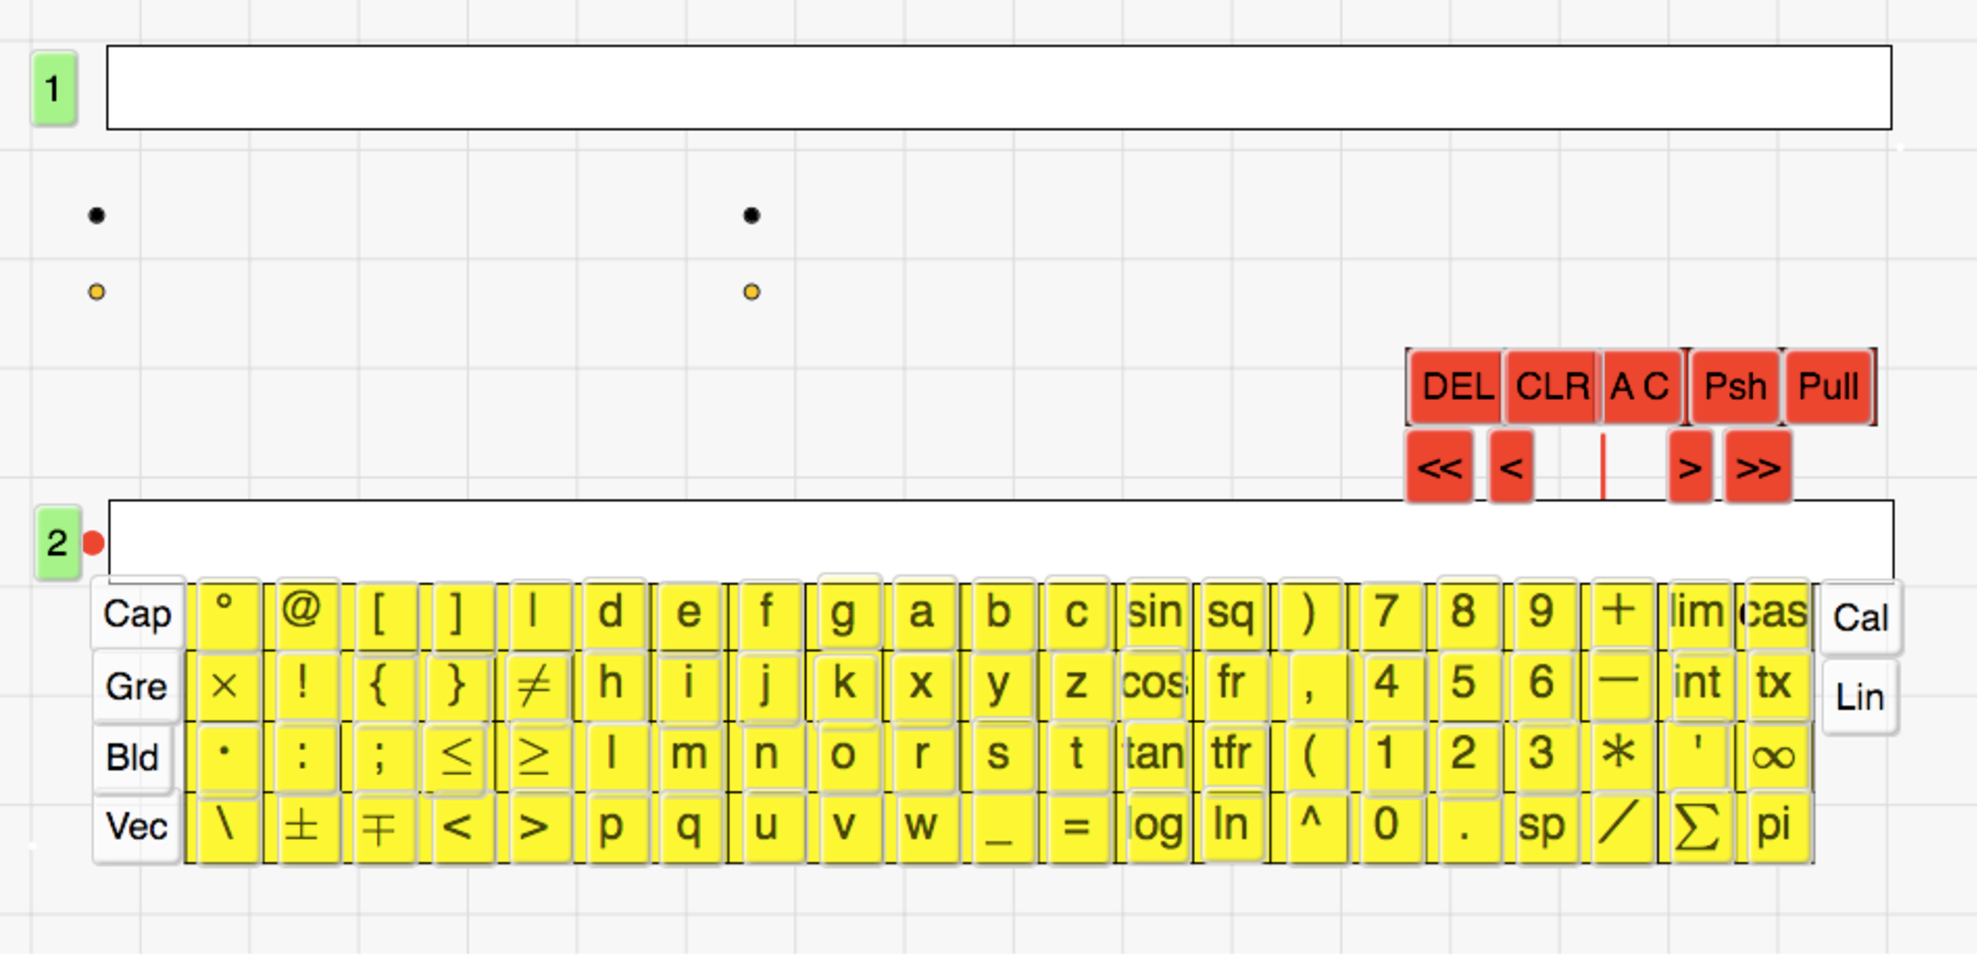
\includegraphics[bb=0.00 0.00 939.00 446.00,height=40mm]{fig/ketmathkey.pdf}}
\arrowlineseg{12}{5}{10}{-135}
\arrowlineseg{12}{24}{10}{135}
\putnotec{5}{14}{\footnotesize 入力窓の切替}
\arrowlineseg{14.5}{27}{8}{180}
\arrowlineseg{14.5}{29}{8}{180}
\putnotew{6}{26.5}{\scriptsize 大文字}
\putnotew{6}{29.5}{\scriptsize ギリシャ}
\arrowlineseg{90}{16}{8}{0}
\arrowlineseg{90}{20}{8}{0}
\putnotee{98}{16}{\scriptsize 入力文字の削除}
\putnotee{98}{20}{\scriptsize 入力ポイントの移動}
\arrowlineseg{12}{40}{3}{-90}
\putnotes{12}{44}{\scriptsize TeXソース}
\arrowlineseg{90}{27}{8}{0}
\arrowlineseg{90}{30}{8}{0}
\putnotee{98}{27}{\scriptsize 微積分}
\putnotee{98}{30}{\scriptsize 線形代数}
\end{layer}

\end{itemize}
%%%%%%%%%%%%%

%%%%%%%%%%%%%%%%%%%%

\mainslide{KeTMathによる課題処理}


%%repeat=3
\slidepage[m]
%%%%%%%%%%%%%

%%%%%%%%%%%%%%%%%%%%

\newslide{準備}

\vspace*{18mm}

%%repeat=3
\slidepage
\begin{enumerate}[(1)]
\item
サブフォルダdataを作成する.
\item
学生リスト(txt)を作成してdataに入れる.\\
 ファイル名は student2021.txtなどとして,1行ずつ名前を入れる.
\item
問題と正解のファイルquestion(+date).txtを作成してdataに入れる.\\
 詳細は次ページ
\end{enumerate}
%%%%%%%%%%%%%

%%%%%%%%%%%%%%%%%%%%

\newslide{問題と解答の作成(question)}

\vspace*{18mm}

%%repeat=3
\slidepage
\begin{itemize}
\item
タイトル行 \verb|Q...|\\
問題文\\
小問(番号は[1]...)\\
Sheet\\
解答欄の作成\\
「\dc」の後に配点を書く\\
Ans\\
解答\\
1行空白行をおく
\item
1つの問題に複数の選択肢を与えるときは\dc (ダブルコロン)で区切る.
\item
ファイル名は\verb|question1030(=date).txt|などとしてdataに入れる.
\end{itemize}
%%%%%%%%%%%%%

%%%%%%%%%%%%%%%%%%%%

\newslide{問題と解答の作成例}

\vspace*{18mm}

%%repeat=3
\slidepage
\begin{itemize}
\item
[]Q10301\\
次の値を求めよ\\
$[1]$ sin(15(deg))\dc sin(75(deg))\\
$[2]$ cos(75(deg)\dc cos(15(deg))\\
Sheet\\
$[1]$= \ \ \dc 5\\
$[2]$= \ \ \dc 5\\
Ans\\
$[1]$ fr(sq(6)-sq(2),4)\dc fr(sq(6)+sq(2),4)\\
$[2]$ fr(sq(6)-sq(2),4)\dc fr(sq(6)+sq(2),4)\\
  (空白行)
\end{itemize}
%%%%%%%%%%%%%

%%%%%%%%%%%%%%%%%%%%

\newslide{問題と解答の作成例(続)}

\vspace*{18mm}

%%repeat=3
\slidepage
\begin{itemize}
\item
[]Q10302\\
sin(x-fr(pi,4))をsin(x),cos(x)で表せ.// Hint : 加法定理を用いよ.\\
Sheet\\
=  \dc 10\\
Ans\\
sin(x)cos(fr(pi,4))-cos(x)sin(fr(pi,4))//=fr(1,sq(2))(sin(x)-cos(x)) \\
\end{itemize}
%%%%%%%%%%%%%

%%%%%%%%%%%%%%%%%%%%

\newslide{taskline.txtの作成}

\vspace*{18mm}

%%repeat=3
\slidepage

\begin{layer}{120}{0}
\putnotese{75}{7}{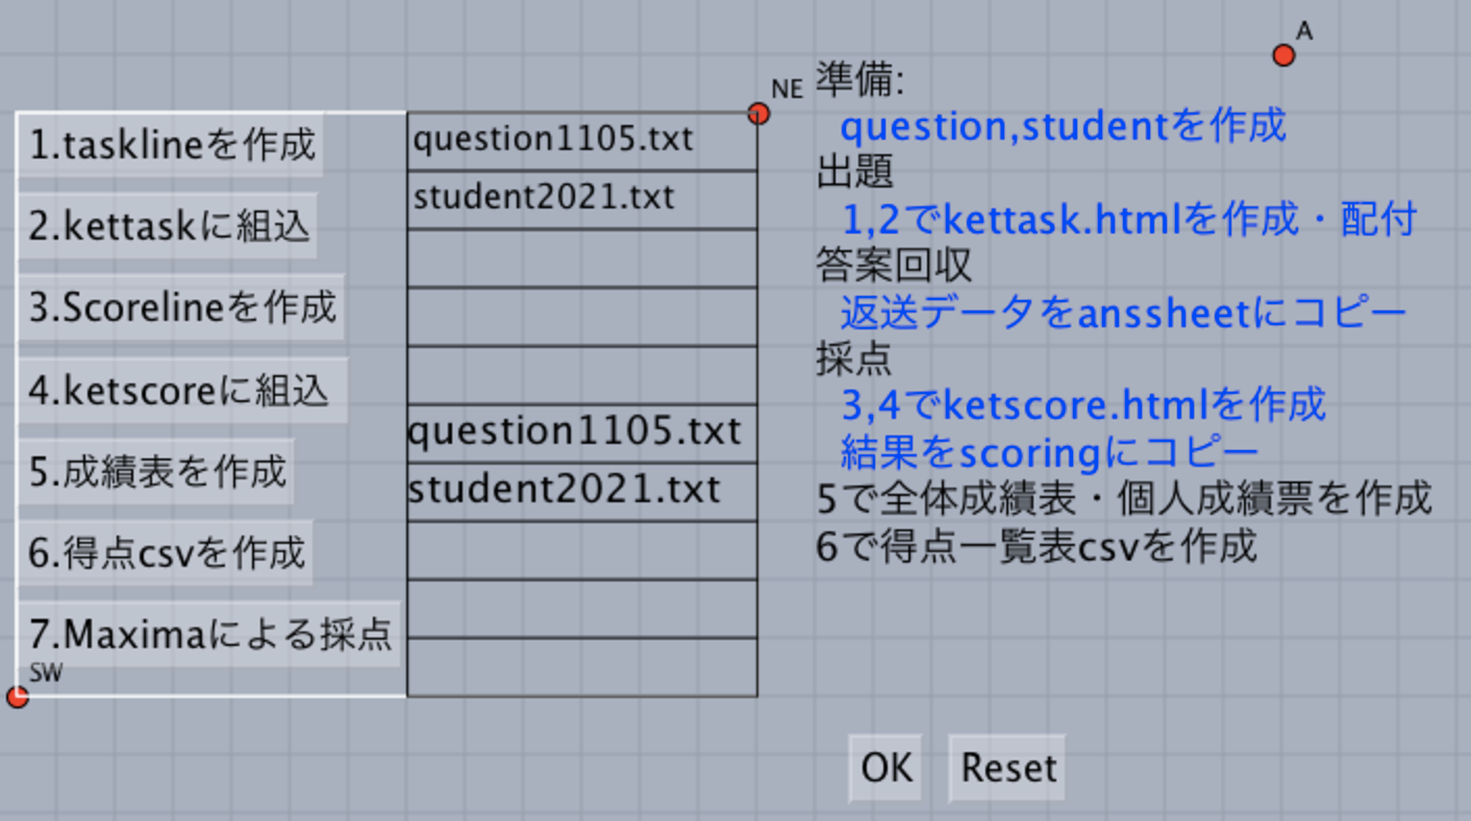
\includegraphics[bb=0.00 0.00 706.00 394.00,width=50mm]{fig/toolketmath.pdf}}
\end{layer}

\begin{itemize}
\item
toolketmath.cdyを立ち上げる.
\item
「1.tasklineを作成」のボタンを押す.\\
 ファイルquestion,studentが表示
\item
それらのファイルを順にクリック\\
 下にファイル名が表示される.
\item
OKボタンを押す.\\
・1tasklineのテキストファイルがdataに作成される.\\
  注)ファイル名にはquestionの日付が付加される.\\
・青字で1tasklineのファイル名が表示される.\\
・学生の解答を入れる2anssheet(+date).txtというファイルもできる
\item
toolketmath.cdyは立ち上げたままにしておく.
\end{itemize}
%%%%%%%%%%%%%

%%%%%%%%%%%%%%%%%%%%

\newslide{kettask.html(課題用)の作成}

\vspace*{18mm}

%%repeat=3
\slidepage
\begin{itemize}
\item
toolketmath.cdyを立ち上げる(終了した場合).
\item
「2.kettaskに組込」のボタンを押す.\\
 ・kettaskorg.htmlと1taskline(+date).txtのファイルが表示される.
\item
それらのファイルを順にクリック\\
 ・右下にファイル名が表示される.
\item
OKボタンを押す.\\
 ・kettask(+date).htmlがカレントディレクトリに作成される.\\
   注)ketaskorgに1tasklineを挿入した課題ファイル(html)である.
\item
このファイルをwebサイトにおき,リンク先を学生に知らせる.\\
 ・これが出題になる.
\end{itemize}
%%%%%%%%%%%%%

%%%%%%%%%%%%%%%%%%%%

\newslide{kettaskの画面}

\vspace*{18mm}

%%repeat=3
\slidepage

\begin{layer}{130}{0}
\putnotes{60}{5}{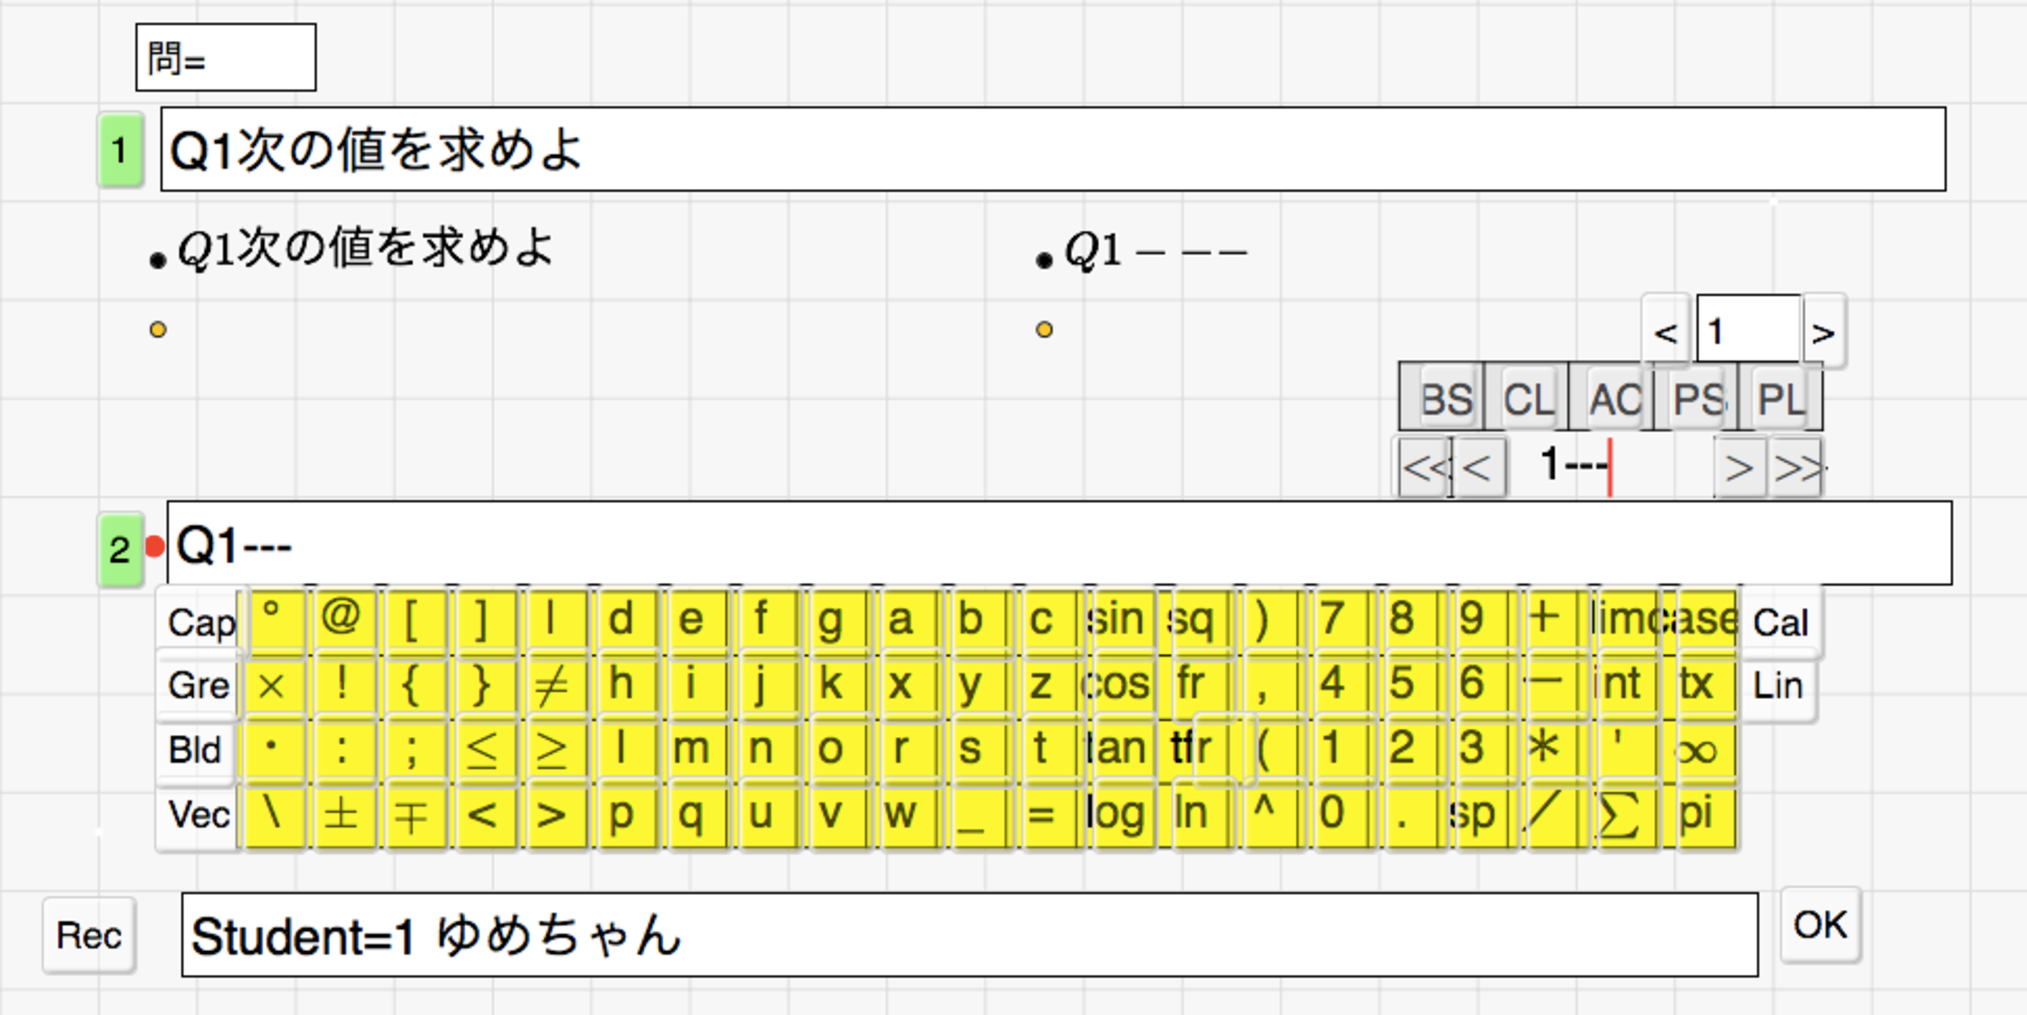
\includegraphics[bb=0.00 0.00 973.00 487.00,width=120mm]{fig/kettask.pdf}}
\arrowlineseg{107}{62}{4}{-90}
\putnotes{107}{66}{\scriptsize 番号を入れてOK}
\arrowlineseg{117}{14}{4}{0}
\putnotee{121}{14}{\scriptsize 問題表示}
\arrowlineseg{112}{24}{4}{0}
\putnotee{116}{24}{\scriptsize ページ}
\arrowlineseg{117}{37}{4}{0}
\putnotee{121}{37}{\scriptsize 解答入力}
\arrowlineseg{5}{63}{4}{-90}
\putnotes{5}{67}{\scriptsize 答案を表示}
\end{layer}

%%%%%%%%%%%%%

%%%%%%%%%%%%%%%%%%%%

\newslide{学生による解答と提出}

\vspace*{18mm}

%%repeat=3
\slidepage
\begin{itemize}
\item
配付されたリンク先をクリック
\item
欄3のStudent=の後に番号をキーボードで入力してOKを押す.
\item
名前を確認して解答用の欄2に答えを入力
\item
赤いボタンの上の窓にページ番号が表示される.\\
・白い矢印を押してページ番号をを変えて.回答する.\\
・「---」のあるページには入力できない.
\item
解答が終わったら,「Rec」ボタンを押すと欄3にすべての解答が入る.
\item
「すべてを選択」>「コピー」\vspace{-2mm}
\item
提出用の欄などにペーストして送信する
\end{itemize}
%%%%%%%%%%%%%

%%%%%%%%%%%%%%%%%%%%

\newslide{scoreline.txtの作成}

\vspace*{18mm}

%%repeat=3
\slidepage
\begin{itemize}
\item
提出された解答をstans(+date).txtにコピーする.\\
 ・GoogleClassroomのデータをそのままコピペしてもよい.\\
 ・不要な行の削除やソーティングはKeTMathが行う.
\item
toolketmath.cdyを立ち上げて,「3.Scorelineを作成」を押す.\\
 ・question, 1taskline, 2anssheetのファイル表示.
\item
それらのファイルを順にクリックすると,右下にファイル名が表示される.
\item
OKボタンを押す.\\
 ・3scorelineのテキストファイルがdataに作成される.\\
   注)ファイル名にはquansの日付が付加される.\\
 ・採点結果を入れるresult(+date).txtというファイルができる
\end{itemize}
%%%%%%%%%%%%%

%%%%%%%%%%%%%%%%%%%%

\newslide{ketscore.html(採点用)の作成}

\vspace*{18mm}

%%repeat=3
\slidepage
\begin{itemize}
\item
toolketmath.cdyを立ち上げて,「4.ketscoreに組込」を押す.\\
 ・ketscoreorg.htmlとscoreline(+date).txtのファイルが表示される.
\item
それらのファイルを順にクリック
\item
OKボタンを押すと,ketscore(+date).htmlがDircdyに作成される.\\
   注)ketscoreorgにscorelineを挿入した採点ファイル(html)である.
\item
ketscore(+date).htmlを立ち上げる\\
 ・上の紫ボタンで学生番号,赤ボタンの上のボタンで問題番号を変える.\\
 ・\dc の後に点数をキーボードで入れる.\\
 ・採点が済んだらRecを押し,欄3の内容を4.scoresheet(+date).txtにコピペ.
\item
採点途中の場合も,4scoresheet(+date).txtにコピペしておく.\\
 ・再開したら,欄3に4scoresheet(+date).txtの内容をコピーする.
\end{itemize}
%%%%%%%%%%%%%

%%%%%%%%%%%%%%%%%%%%

\newslide{ketscoreの画面}

\vspace*{18mm}

%%repeat=3
\slidepage

\begin{layer}{130}{0}
\putnotese{2}{9}{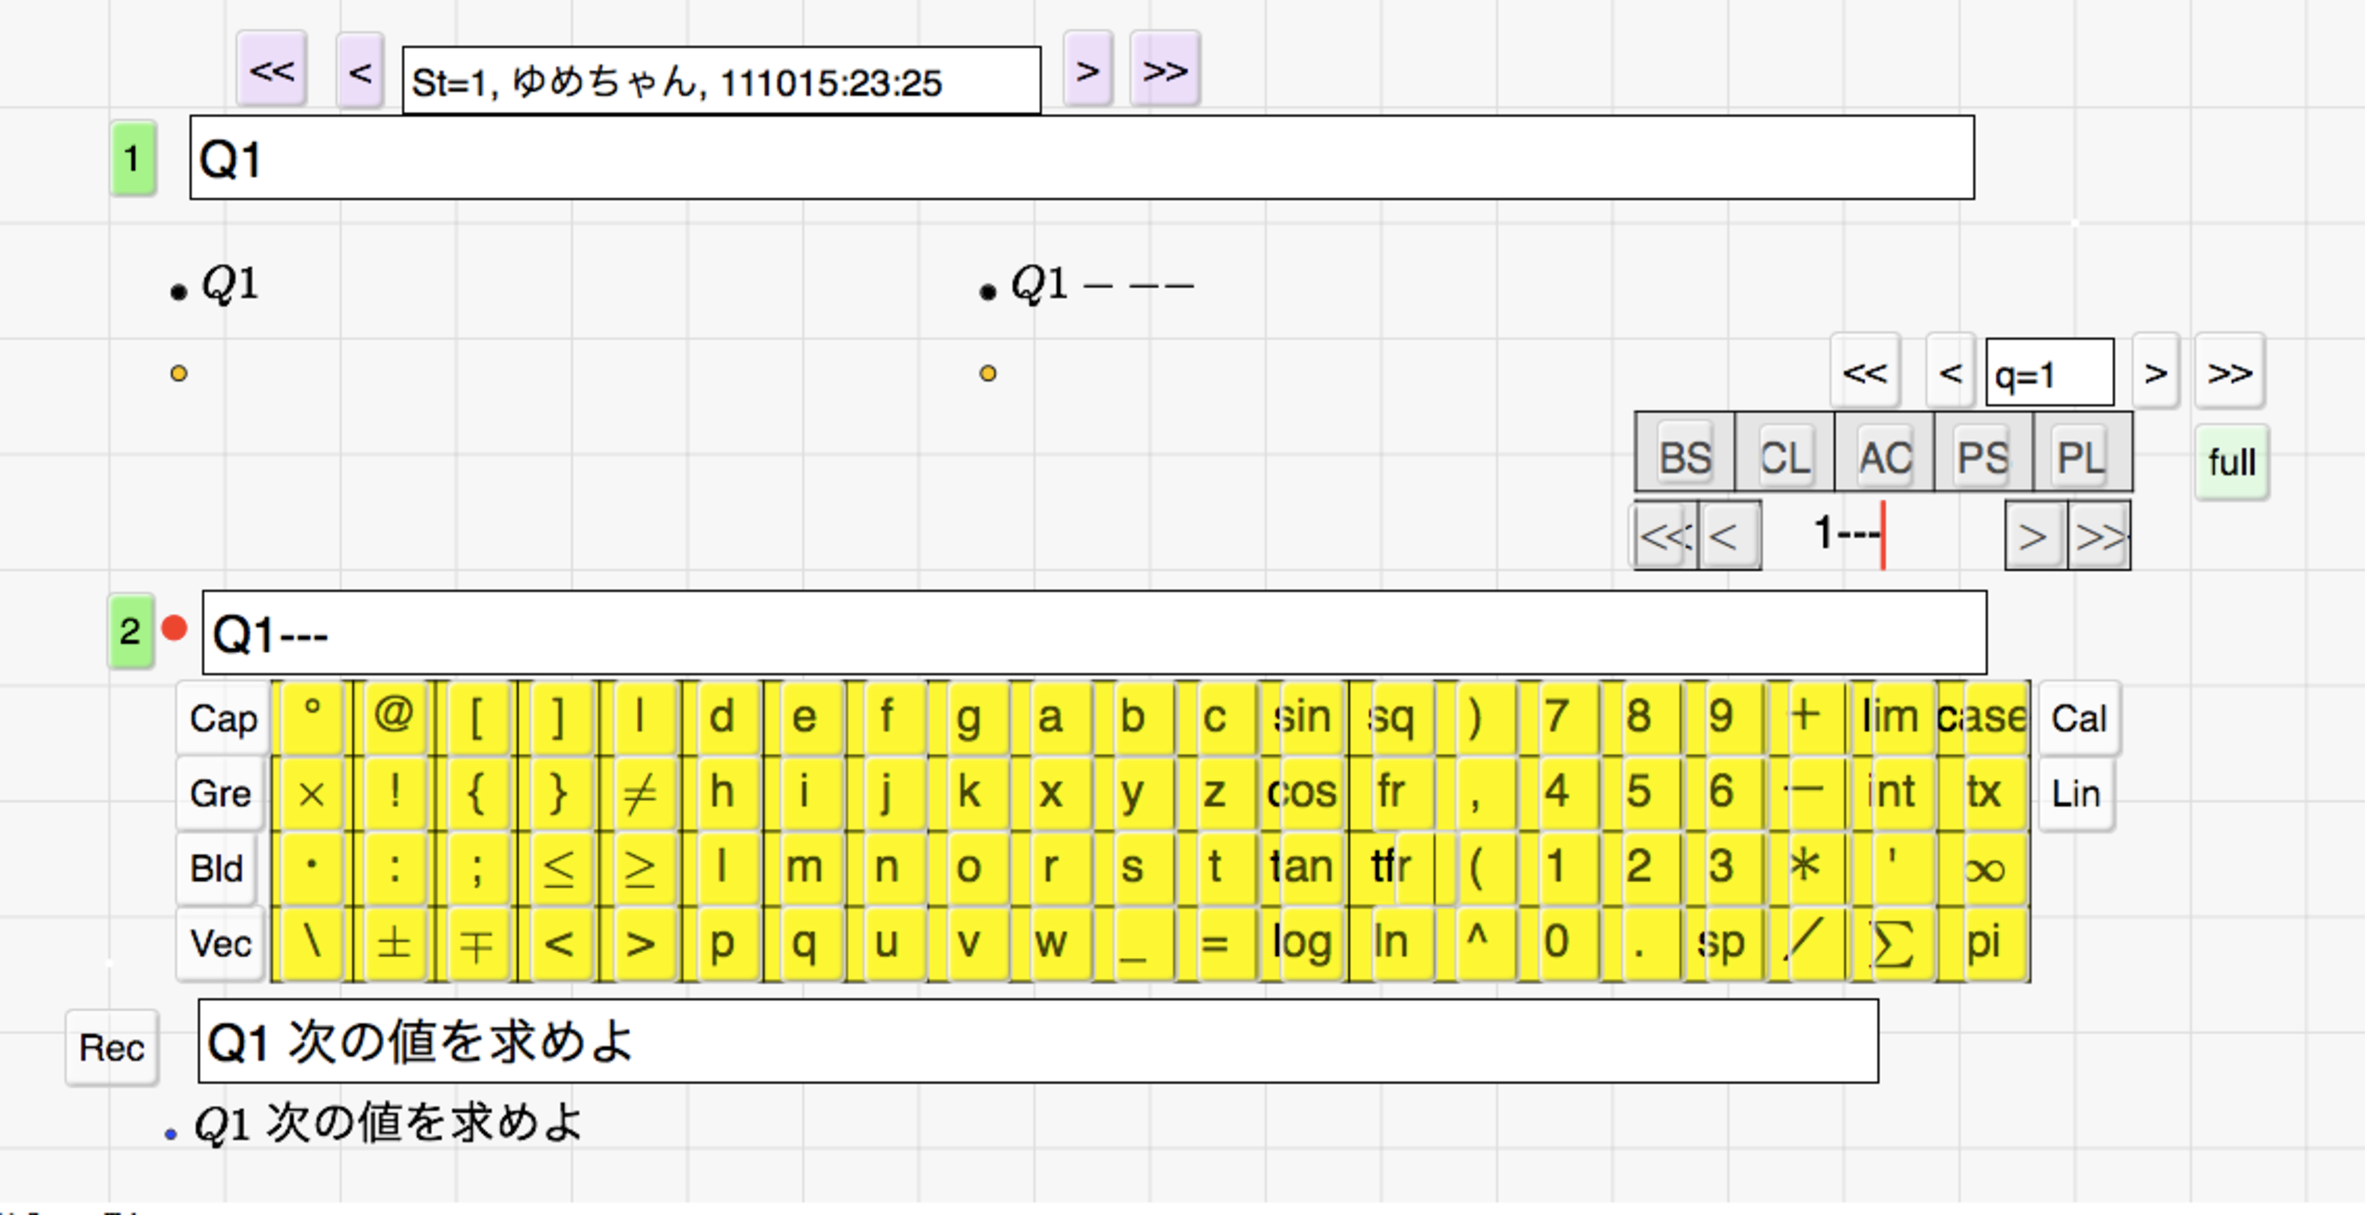
\includegraphics[bb=0.00 0.00 1104.00 564.00,width=115mm]{fig/ketscore.pdf}}
\arrowlineseg{95}{60}{4}{0}
\putnotee{99}{60}{\scriptsize 問題表示}
\arrowlineseg{101}{16}{4}{0}
\putnotee{105}{16}{\scriptsize 正解表示}
\arrowlineseg{113}{27}{4}{0}
\putnotee{118}{27}{\scriptsize ページ}
\arrowlineseg{113}{32}{4}{0}
\putnotee{118}{32}{\scriptsize 満点入力}
\arrowlineseg{101}{40}{4}{0}
\putnotee{105}{40}{\scriptsize 採点入力}
\arrowlineseg{6}{63}{6}{-90}
\putnotes{6}{69}{\scriptsize 結果を欄3に表示}
\arrowlineseg{60}{12}{4}{0}
\putnotee{64}{12}{\scriptsize 学生を表示}
\end{layer}

%%%%%%%%%%%%%

%%%%%%%%%%%%%%%%%%%%

\newslide{配付用成績表と得点一覧ファイルの作成}

\vspace*{18mm}

%%repeat=3
\slidepage
\begin{itemize}
\item
toolketmath.cdyを立ち上げる.
\item
「5.成績票を作成」より,次のファイルが作成される.\\
 ・data/cardに成績票(学生ごと)ファイル\\
 ・dataに全員の成績票をまとめた5recordlist(+date).txt
\item
「6.得点csvを作成」より\\
 dataに得点データのcsvファイル6scoretable1105(+date).csv\\
が作成される.
\end{itemize}
%%%%%%%%%%%%%

%%%%%%%%%%%%%%%%%%%%

\newslide{Maximaによる採点}

\vspace*{18mm}

%%repeat=3
\slidepage
\begin{itemize}
\item
Maximaで採点しない問題には,Sheetの最後に\dc と$-1$をつける\\
   Sheet\\
   [1]=  \dc 5\dc $-1$\\
   [2]=  \dc 5\dc $-1$
\item
「7.Maximaの採点」を押すと,Maximaが起動して採点表\\
   7scoremax(+date).csv\\
ができる
\end{itemize}
\label{pageend}\mbox{}

\end{document}
